\documentclass[english,10pt]{article}
\usepackage{geometry}
\usepackage{hyperref}
\usepackage{inputenc}
\geometry{verbose,tmargin=3.5cm,bmargin=4cm,lmargin=3.8cm,rmargin=3.8cm}
\usepackage[backend=biber,style=ieee]{biblatex}
\addbibresource{sources.bib}
\makeatletter
\usepackage{url}
\usepackage{graphicx}
\usepackage{caption}
\usepackage{wrapfig}
\usepackage{subcaption}
\makeatother
\usepackage{babel}
\usepackage{amsmath}
\usepackage{amsthm}
\newtheorem{theorem}{Theorem}[section]
\newtheorem{lemma}[theorem]{Lemma}
\newtheorem{conjecture}{Conjecture}
\newtheorem{property}{Property}
\newtheorem{corollary}{Corollary}[property] % Use theorem counter as `parent`
\usepackage{algorithm}
\newcommand{\Desc}[2]{\State \makebox[2em][l]{#1}#2}
\usepackage[noend]{algpseudocode}
\makeatletter
\def\BState{\State\hskip-\ALG@thistlm}
\makeatother

\begin{document}
	
	\title{Multi-Agent Path Finding with Matching using Increasing Cost Tree Search}
	
	\author{Thom van der Woude\and Jesse Mulderij\and Mathijs de Weerdt}
	\date{\today}
	
	\maketitle
	
	\begin{abstract}
		Both the assignment problem and the multi-agent pathfinding problem are common problems in the fields of robotics and transportation. The joint problem of multi-agent pathfinding extended with the assignment of goals to agents, matching, is something that has not been studied much; few methods exist today that solve it. In this work, two types of algorithms based on the Increasing Cost Tree Search algorithm for multi-agent pathfinding are presented that can optimally solve this joint problem: exhaustive algorithms that reduce the problem to solving many MAPF problems using regular Increasing Cost Tree Search, and algorithms that search a generalized increasing cost tree. These are compared to each other experimentally on a set of grid maps, and it is shown that exhaustive methods typically outperform the generalized ICT search. Lastly, an exhaustive algorithm is compared to alternative algorithms based on other multi-agent pathfinding approaches to put its performance into the broader context of algorithms for multi-agent pathfinding with matching.
	\end{abstract}
	
	\section{Introduction}
	The Dutch Railways company (NS) needs to clean and service their fleet of trains during the night in shunting yards so that they can properly bring passengers from A to B during the day. 
	The problem of scheduling the trains and personnel to achieve this is called the Train Unit Shunting and Servicing (TUSS) problem \cite{mulderij2020}. 
	It is an NP-hard problem with many different subproblems in addition to the basic train unit routing, such as the timetabling of personnel and coupling and decoupling of train units entering and leaving the yard. % introduce heuristics here.
	
	As was shown by Geiger et al.\cite{geiger2018}, in practical scenarios, only heuristic methods can solve TUSS instances. 
	Such methods are suboptimal and heuristic solutions to instances defined for a set shunting yard can be said to characterise a lower bound on the capacity of the shunting yard, as each solution cost gives a (loose) upper bound for the optimal solution cost. 
	The railway company, however, is interested in learning tight upper bounds for the capacity of existing shunting yards to inform decisions about matters like infrastructure expansion. \cite{mulderij2020} proposes the multi-agent pathfinding (MAPF) problem \cite{stern2019} extended with a matching subproblem (hereafter MAPFM) as a suitable relaxation of (discretised) TUSS for finding such upper-bounds using an approach analogous to that outlined above.
	For this to succeed, a way to optimally solve MAPFM instances is needed, where optimal is defined as minimizing the Sum of Individual Costs (SIC) objective.
	
	Little to no research has been done on MAPFM and solving it optimally. For MAPFM with a makespan objective instead of SIC, known as the combined  target-assignment  and  path-finding (TAPF) problem, there is the Conflict-Based Min-Cost-Flow (CBM) algorithm by Ma and Koenig \cite{ma2016} and a similar approach described in \cite{henkel2019}. Ma and Koenig's method builds upon the conflict-based search method and in particular on the Meta-Agent variation thereof also discussed in \cite{sharon2015} as a high-level search framework; in the low-level search, the connection between anonymous MAPF problems and max-flow problems (as discussed in \cite{yu2013}) is exploited to plan single teams in polynomial time. 
	
	The experiments reported in \cite{ma2016} indicate that this method scales very well as the number of agents and the sizes of teams increase; however, because only 10\% of tiles is blocked in some of the grid maps they use and despite the fact that CBM performance on Kiva\cite{wurman2007} instances is also discussed, it remains to be seen how CBM performs in scenarios with more obstacles and more maze-like scenarios as included in the Moving AI benchmarks \cite{sturtevant2012} for MAPF.
	Nonetheless, the successful application of CBS to solving TAPF begs the question: \textit{can MAPF algorithms such as Increasing Cost Tree Search (ICTS) \cite{sharon2011} or M* \cite{wagner2011} serve as the basis for a MAPFM algorithm?}
	
	\begin{wrapfigure}[19]{R}{.25\textwidth}
		\begin{minipage}{\linewidth}
			\centering\captionsetup[subfigure]{justification=centering}
			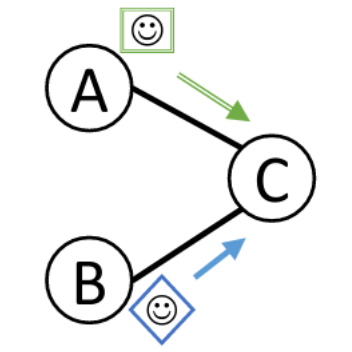
\includegraphics[width=\linewidth]{img/vertex-conflict}
			\subcaption{Vertex conflict}
			\label{fig:conflictsa}\par\vfill
			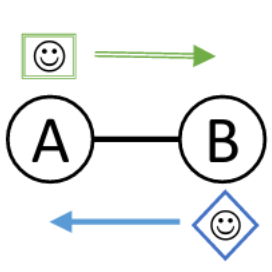
\includegraphics[width=0.75\linewidth]{img/edge-conflict}
			\subcaption{Edge conflict}
			\label{fig:conflictsb}
		\end{minipage}
		\vspace{-10pt}
		\caption{The two types of conflict (from Fig. 1 in \cite{stern2019})}\label{fig:conflicts}
	\end{wrapfigure}
	This work is the outcome of a search for algorithms which optimally solve MAPFM based on ICTS \footnote{To the knowledge of the author, to date, no such algorithm is described in the literature}, which is part of a study in which other algorithms addition to ICTS were taken as starting points for MAPFM algorithms. Two classes of ICTS-based algorithms were found: one based on exhaustive enumeration of matchings using a variant of ICTS as a subroutine, the other based on modifications to the ICT structure and its search. One exhaustive ICTS algorithm is compared to algorithms based on CBM \cite{ma2016}, M*\cite{wagner2011}, A*+OD+ID\cite{standley2010} and EPEA*\cite{goldenberg2014} respectively to put ICTS methods for MAPFM into a broader context.
	
	\section{Multi-agent pathfinding with matching} % Problem description
	\label{mapfm}
	The MAPFM problem is an extension of MAPF, a well-studied problem. Formally, a MAPF instance can be described as follows. Let $G = (V,E)$ be an undirected connected graph, with each $v\in V$ representing an obstacle-free tile on a 4-connected grid and each $e = (u,v)\in E$ representing a legal uniform-cost move between two such tiles. Let there be $k$ agents $a_1,\ldots,a_k$ with starting locations $s_1,\ldots,s_k$ and goals $g_1,\ldots,g_k$. For each agent $a_i$, a path $\pi_i$ from $s_i$ to $g_i$ is to be found such that all agents paths $\pi_i$ taken together are non-conflicting and therefore are a solution. In this work, non-conflicting means, in the conflict-terminology of \cite{stern2019}, that there are no vertex conflicts (and thus no edge conflicts) and no edge conflicts, as shown in Figure \ref{fig:conflicts}. Letting $\pi_i^t$ denote the $t$'th node of path $\pi_i$, this means that for $i\neq j$, for all $t$, $\pi_i^t\neq \pi_j^t$ and $(\pi_i^t \neq \pi_j^{t + 1})\lor(\pi_i^{t+1} \neq \pi_j^t)$. Given a solution $(\pi_1,\ldots,\pi_k)$, a vector of per-agent costs $(c_1,\ldots,c_k)$ can be found. For $\pi_i$, $c_i$ is defined as the time at which $a_i$ reaches $g_i$ for the last time and remains there, meaning that for $t \geq c_i$, $\pi_i^{t} = g_i$. One property of $c_i$ is that $c_i \geq c^*_i$ where $c^*_i$ is defined as the cost of $\pi^*_i$, the shortest path from $s_i$ to $g_i$ that can be computed using any optimal pathfinding algorithm. There are two common objectives in MAPF:
	\begin{itemize}
		\item The makespan: $\max_{i} c_i$
		\item The sum of individual costs (SIC): $\sum_i c_i$
	\end{itemize}
	In this work, following the definition of the TUSS relaxation in \cite{mulderij2020}, an optimal solution is defined as having minimal SIC. Note that $\sum_i c_i \geq \sum_i c^*_i$.
	\begin{wrapfigure}[10]{R}{.35\textwidth}
		\vspace{-10pt}
		\centering
		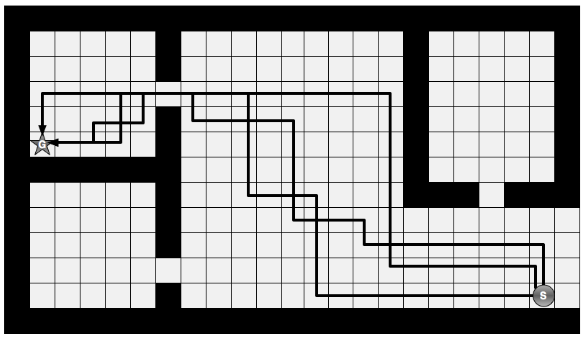
\includegraphics[width=\linewidth]{img/symmetries}
		\caption{Symmetric paths on a 4-connected grid\cite{harabor2010}}
		\label{fig:symmetries}
	\end{wrapfigure}
	The mapping from $(\pi_1,\ldots,\pi_k)$ to a SIC is surjective: many cost vectors $(c'_1,\ldots,c'_k)$ might add up to the same SIC as $(c_1,\ldots,c_k)$ and for a given agent $a_i$, there might be many equivalent paths $\pi'_i$ to the goal with cost $c_i$. On uniform-cost 4-grids in particular, there are often many equivalent and symmetrical paths\cite{harabor2010} (see Figure \ref{fig:symmetries}), which is why in single-agent pathfinding, symmetry-breaking methods such as Jump Point Search\cite{harabor2011} are used to speed up the search. In multi-agent pathfinding, having multiple paths per agent of the same cost can, in contrast, be a boon: it means that there are potentially more non-conflicting ways to combine paths of different agents.
	
	\subsection{Extending MAPF with matching}
	With the multi-agent pathfinding problem defined, the matching extension of MAPF (MAPFM) that is the subject of this paper can be described. The ICTS algorithm for MAPF and possible matching extensions of ICTS will be discussed in Section \ref{section:icts-matching}.
	
	Let there be $K$ teams $t_1,\ldots, t_K$, where $t_i$ consists of $k_i$ agents with start positions $s_1^i,\ldots,s_{k_i}^i$ together with an equal number of team goals $g_1^i,\ldots,g_{k_i}^i$. Within each team $t_i$, agents $a_j^i$ are to be \textit{matched} to a unique goal $g_k^i$, so that exactly one agent is assigned to each goal within team $i$; once all agents are matched to goals, for each agent $a_j^i$ matched to $g_k^i$, a path from $s_j^i$ to $g_k^i$ is to be found such that all agents paths taken together are non-conflicting and therefore make up a solution, similarly defined as for MAPF.
	
	As discussed in \cite{ma2016}, MAPFM generalizes both MAPF and anonymous MAPF, which is MAPF allowing an agent to move to any goal, a problem that can be solved in polynomial time.
	\section{Solving MAPF with Matching using ICTS} % Your contribution
	\label{section:icts-matching}
	Taking ICTS for MAPF as starting point, two methods to use ICTS for MAPFM were identified. The first method relies on a reduction from MAPFM to repeated MAPF: an optimal solution to MAPFM corresponds to a matching of agents to goals, so by exhaustively enumerating all matchings and solving these as MAPF instances, an optimal solution to the MAPFM instance can be found. In the second method, the increasing cost trees search itself is modified to allow an agent $a_j^i$ to be matched to any $g_k^i$. First, ICTS for MAPF and some common variants will be described. Next, derived MAPFM algorithms are introduced and properties of these algorithms and some variants are discussed. In Section \ref{experiments}, these will be compared experimentally.
	\subsection{Increasing Cost Tree Search}
	\label{icts}
	In Increasing Cost Tree Search\cite{sharon2011}, the two-step mapping from path combination to SIC described in Section \ref{mapfm} is reversed to search for a solution with minimal SIC. This is done by searching for cost vectors corresponding to increasing SIC on the top level and searching for non-conflicting path combinations (solutions) for each cost vector on the bottom level. 
	
	\subsubsection{Top-level search}
	In the top-level search, all possible cost vectors for a given SIC are evaluated by searching an Increasing Cost Tree as depicted in \ref{fig:ict}, starting from $C^* = \sum_i c^*_i$ corresponding to a single root cost vector $(c^*_1,c^*_2,\ldots,c^*_k)$. This root has $k$ children $(c^*_1 + 1,c^*_2,\ldots,c^*_k),(c^*_1,c^*_2 + 1,\ldots,c^*_k),\ldots,(c^*_1,c^*_2,\ldots,c^*_k + 1)$ all of cost $C = C^* + 1$. Searching this ICT breadth-first corresponds to evaluating all possible cost vectors corresponding to increasing cost $C$ starting with $C^*$, guaranteeing optimality of a found solution. The number of cost vectors evaluated when searching up to nodes of cost $C^* + \Delta$ is $\mathcal{O}(k^\Delta)$. Node evaluation is done by a low-level search that searches for a solution $(\pi_1,\ldots,\pi_k)$ corresponding to the node costs $(c_1,\ldots,c_k)$.
	
	\begin{figure}[t]
		\centering
		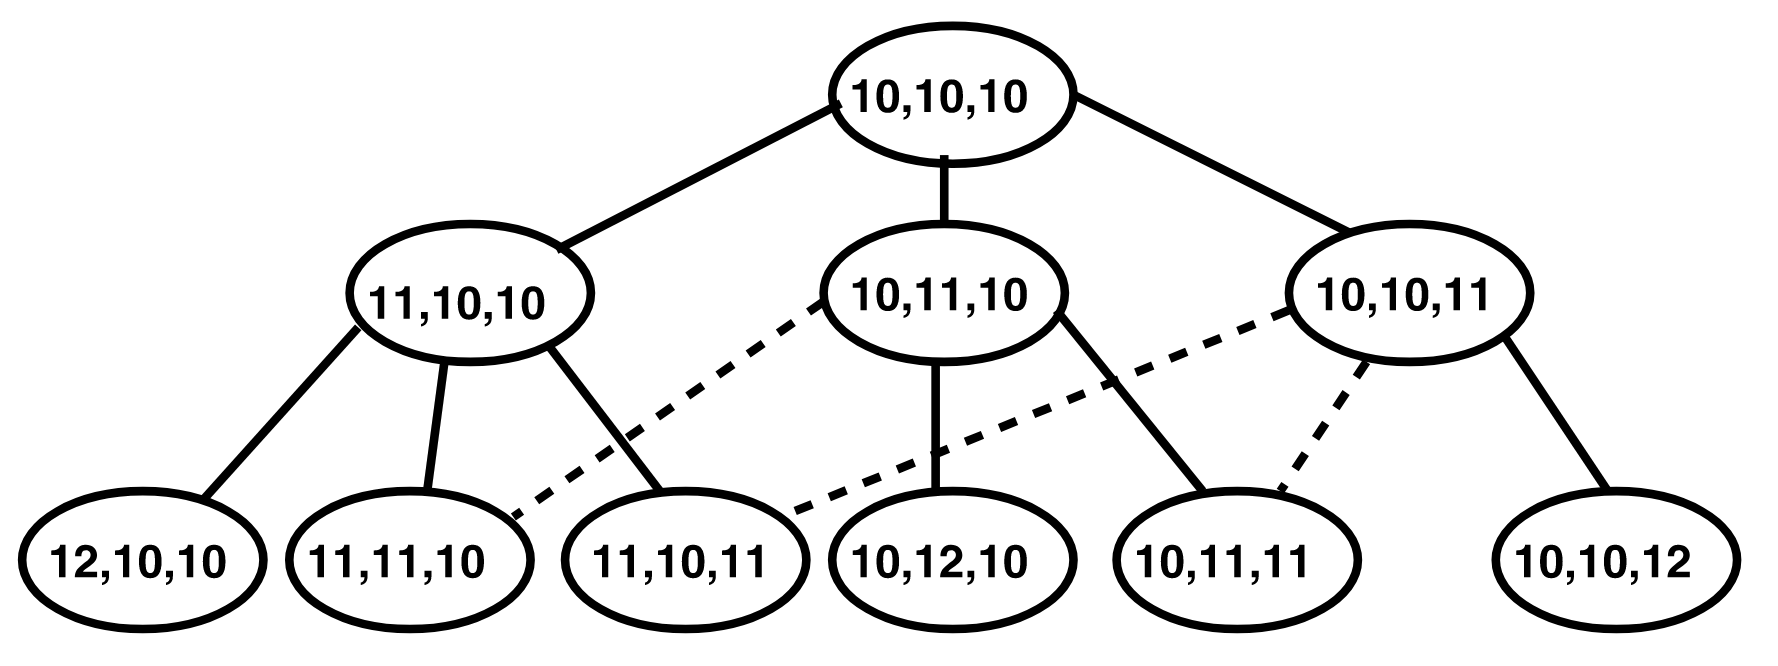
\includegraphics[width=0.5\linewidth]{img/ict}
		\caption{Increasing Cost Tree for three agents \cite{sharon2011}}
		\label{fig:ict}
		\vspace{-30pt}
	\end{figure}
	\begin{figure}
		
	\end{figure}
	
	
	\begin{figure}[b]
		\centering
		\begin{subfigure}{0.2\textwidth}
			\centering
			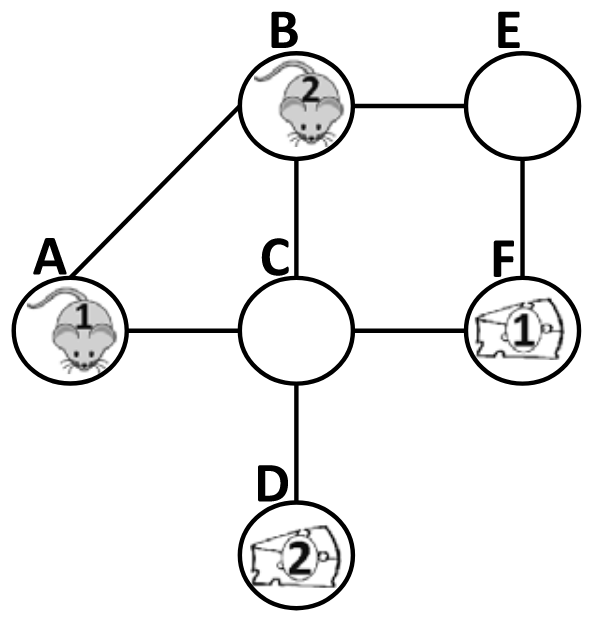
\includegraphics[width=\linewidth]{img/mdds1}
			\caption{An example problem}
			\label{fig:problem}
		\end{subfigure}
		\hfill
		\begin{subfigure}{0.3\textwidth}
			\centering
			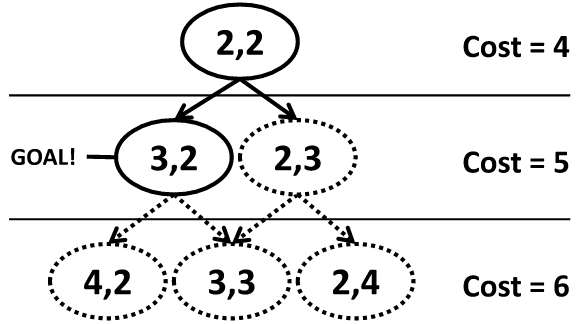
\includegraphics[width=\linewidth]{img/ict2}
			\caption{The corresponding ICT with solution node $(3,2)$}
			\label{fig:ict2}
		\end{subfigure}
		\hfill
		\begin{subfigure}{0.4\textwidth}
			\centering
			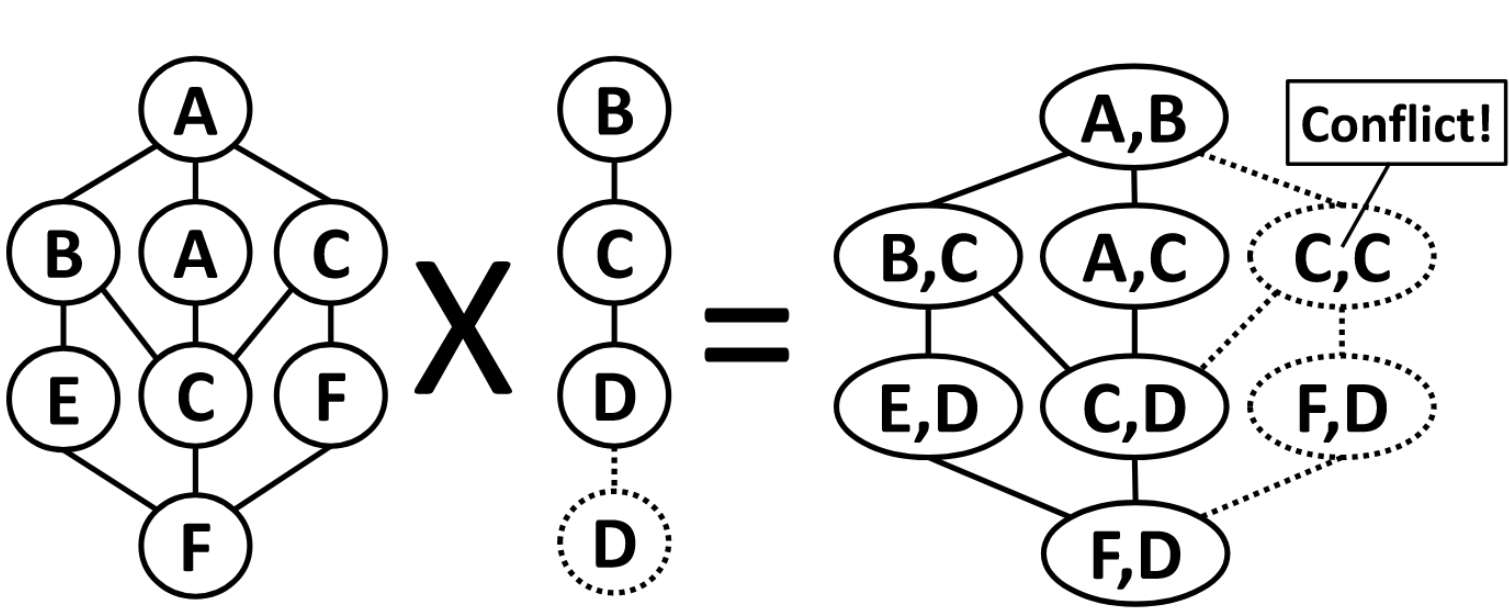
\includegraphics[width=\linewidth]{img/mdds}
			\caption{MDDs for the agents are found and combined}
			\label{fig:mdds}
		\end{subfigure}
		
		\caption{Example of using ICTS to solve MAPF from \cite{sharon2011}}
		\label{fig:bottom}
	\end{figure}
	\subsubsection{Bottom-level search}
	Explicitly generating all paths to the goal for agent $a_i$ of cost $c_i$ is expensive: the number of paths is exponential in $c_i$. This is why in the low-level search of ICTS, multi-valued decision diagrams (MDDs) are used to compactly represent all paths per agent. For $a_i$ with a target cost $c_i$ (from the cost vector), $MDD_i^{c_i}$ can be generated by a breadth-first search on the $c_i$-steps time-expanded graph starting at $s_i$, followed by a process similar to the standard path reconstruction method used in A* but allowing multiple node parents. Storing the resulting paths in an MDD, which has at most $|V|$ nodes at each timestep or depth, avoids the cost of storing all paths explicitly and facilitates the efficient search of the $k$-agent space of path combinations \cite{sharon2011}.
	
	In Figure \ref{fig:bottom}, a problem with its corresponding ICT is shown, as well as the low-level search of the (solution) node $(3,2)$ using MDDs. Note that the second agent staying at node D after completing the path is modelled in its MDD also to ensure that the place remains blocked.
	
	Subfigure \ref{fig:mdds} illustrates how two or more MDDs can be combined: first, the root nodes are joined; next, the product of the children of both roots is taken and checked for conflicts. In \ref{fig:mdds}, a vertex conflict occurs and therefore this joint child can be removed from the MDD. If a $(B,A)$ node would be generated by the same root, $(A,B)$, this would similarly be an edge conflict and hence $(B,A)$ would also be removed from the joint MDD $MDD_{1,2}^{c_1,c_2}$. In the next layer, the process repeats with multiple parent nodes.
	
	In practice, joint MDDs are not explicitly constructed but instead, a depth-first search is used to search joint MDDs. This has the benefit of finding a path to the bottom of the joint MDD fast if one exists, while not constructing more of the joint MDD (which can get rather large) than is necessary for finding a solution.
	\subsubsection{ICTS with Independence Detection}
	Like other MAPF algorithms, ICTS can be embedded in the Independence Detection (ID) framework introduced by Standley in \cite{standley2010}. ID starts by assuming each agent is a group that can be assigned an optimal path independent of other groups. If group paths do conflict, they become one group that is planned together using a MAPF algorithm, in this case, ICTS, until no conflicts between groups occur. The goal of ID is to minimize $k'$, the size of the largest group that has to be planned. Optionally, a conflict avoidance table (CAT) can be maintained for use during the planning of groups. This records the paths planned by other groups and can facilitate tie-breaking in search that minimizes the number of conflicts; the CAT is omitted from Algorithm \ref{id-algo} for brevity but was implemented and used in experiments.
	\begin{algorithm}
		\begin{algorithmic}[1]
			\State \text{Assign each agent to a singleton group}
			\State \text{plan a path for each group}
			\Repeat
			\State \text{simulate execution of all paths until a conflict occurs}
			\State \text{merge two conflicting groups into a single group}
			\State \text{cooperatively plan new group}
			\Until{\text{no conflicts occur}}
			\State $solution\gets\text{paths of all groups combined}$
			\State \textbf{return solution}
		\end{algorithmic}
		\caption{Simple Independence Detection \cite{standley2010}} 
		\label{id-algo}
	\end{algorithm}
	\subsubsection{Pruning in ICTS}
	\label{pruning}
	In \cite{sharon2011}, in addition to the basic two-level solver, three pruning methods to speed up search are discussed, two of which were used in this work. All work by taking $j < k$ and applying the described method to each possible combination of $j$ out of $k$ agents. If no solution exists for any such combination, the full $k$-agent low-level search is not triggered. The two basic pruning methods are as follows.
	\begin{enumerate}
		\item Simple pruning: the $j$-agent MDD is searched using DFS for a solution.
		\item Enhanced pruning: the $j$-agent MDD is searched using BFS and when children are generated, for each agent, all children that do not appear in any unified node are removed from the MDD. In \ref{fig:mdds}, the $C$ node of $MDD_1$ would be removed as it cannot be unified with any node of $MDD_2$ at that level. 
	\end{enumerate}
	In addition, repeated enhanced pairwise pruning is described in which the enhanced pruning procedure is repeated for all combinations until a fixpoint is reached, which is when no child node is removed from any of the agent MDDs in an iteration. This was not used in this work. 
	
	The full ICT-search algorithm including a pruning step is described by Algorithm \ref{icts-algo}. It is reproduced from \cite{sharon2011} for completeness. As noted before, this procedure can be used for planning groups in Algorithm \ref{id-algo}. In this work, triple-pruning was used and enhanced triple-pruning was taken as a baseline, as the conclusion in \cite{sharon2011} is that this often outperforms other variants.
	\begin{algorithm}
		\begin{algorithmic}[1]
			\Procedure{ICT-search}{MAPF instance}
			\State \text{Construct ICT root}
			\ForAll{\text{ICT nodes }$(c_1,\ldots,c_k)$\text{ in breadth-first order }} 
			\ForAll{\text{agents} $a_i$} 
			\text{Construct} $MDD_i^{c_i}$
			\EndFor
			\ForAll{$j$-\text{agent combinations} $(i_1,\ldots,i_j)$} 
			\State \text{Run node-pruning procedure with MDDs }$MDD_{i_1}^{c_{i_1}},\ldots,MDD_{i_j}^{c_{i_j}}$
			\If{\text{no solution was found for a combination in pruning}}
			\State \textbf{Break}\text{ and continue with next ICT node}
			\EndIf
			\EndFor
			\State \text{Search }$k$\text{-agent MDD space}
			\If{\text{solution was found}}
			\State \textbf{return solution}
			\EndIf
			\EndFor
			
			\EndProcedure
		\end{algorithmic}
		\caption{Increasing Cost Tree Search}
		\label{icts-algo}
	\end{algorithm}
	\subsection{Exhaustive ICTS}
	\label{exhaustive}
	For $K$ teams $t_1,\ldots,t_K$ of size $k_i$, there are in total $M = \prod_{i} k_i!$ matchings from team agents to team goals. Let $C_1$ through $C_M$ denote the optimal SIC costs of each MAPF instance corresponding to the instance, with $C_m = \infty$ for infeasible $m$. In order to find the optimal solution, $m$ with lowest $C_m$ has to be found, which requires all $M$ to be solved or found to be unfeasible, meaning that $\mathcal{O}(M)$ MAPF instances have to be solved. 
	\subsubsection{Bounded search}
	Once the first solution is found with cost $C$, this can be used in the next search as an (exclusive) upper-bound $B$ for the SIC of nodes that have to be searched. Formally, let $B_0 = \infty$ represent the initial SIC bound of the ICT search. After solving each $m$ with solution cost $C_m$, let $B_{m+1} = \min(B_m,C_m)$. By successively updating this $B$ in this manner, as more matchings are solved, the effort needed to solve the remaining matchings can be expected to be reduced significantly. With $C_m$ denoting the optimal SIC for matching $m$, this effort can be expressed as	
	\[\Delta_{m,\text{bounded}} = \min(B_m,C_m) - C^*_m = B_{m+1} - C^*_m\]
	This is proportional to the effort due to the complexity of the ICTS search for matching $m$, $\mathcal{O}(k^{\Delta_{m,\text{bounded}}})$.
	If $B_m < C^*_m$, only the root node will be generated to determine this so $\Delta_{m,\text{bounded}} = 0$.
	Using this, the number of ICT nodes searched in total becomes $\mathcal{O}(\sum_m k^{\Delta_{m,\text{bounded}}})$.
	\subsubsection{Ordered enumeration}
	\label{ordered-enum}
	To reduce the total effort as much as possible, the matchings $m$ can be enumerated and solved in increasing order of $C^*_m$. In this case, the effort per matching is monotonically non-increasing by Property \ref{monotonicity}. This induces a case in which this enumeration minimizes the number of nodes searched in total (Property \ref{cond-monoton-optim}). However, cases in which $\Delta_m$ of the first $m$'s searched is much higher could also be constructed, in which case this approach might cause more nodes to be processed in total than alternative methods. Therefore, this ordered enumeration remains a heuristic improvement that works well in practice, as shown in Section \ref{experiments}.
	
	\begin{property}[Monotonicity]
		\label{monotonicity}
		In bounded exhaustive search using ICTS, solving the matchings in increasing order of root SIC makes the effort $\Delta_{m,\text{bounded}}$ monotonically non-increasing as a function of $m$.
	\end{property}
	\begin{proof}
		Due to the order of matchings for successive matchings $m,m+t$ for some $t\geq 1$, $C^*_{m} \leq C^*_{m+t}$. By definition, $B_{m+2} = \min(B_{m+1},C_{m+1})$ meaning that $B_{m+2} \leq B_{m + 1}$ so transitively $B_{m+t+1} \leq B_{m+1}$. Therefore
		\[B_{m+t+1} - C^*_{m+t}\leq B_{m+1} - C^*_m\implies \Delta_{m+t,\text{bounded}} \leq \Delta_{m,\text{bounded}}\]
	\end{proof}
	\begin{property}[Conditional optimality]
		\label{cond-monoton-optim}
		Assuming that $\Delta_m$, the unbounded effort, is monotonically non-decreasing as a function of $m$ (with $m$ in increasing order of $C^*_m$), ordered enumeration minimizes the total number of nodes searched across matchings.
	\end{property}
	\subsubsection{Approximate ordered enumeration}
	In practice, it is difficult enumerate all matchings in increasing order of root SIC. Finding a lowest SIC $m$ reduces to the assignment problem that can be solved using the Hungarian algorithm \cite{kuhn55} in polynomial time; however, to the knowledge of the author, no algorithm exists to more generally compute the $i$'th matching in increasing order of $C^*_m$ (assuming some fixed tie-breaking). This means that matchings have to be exhaustively enumerated and stored in memory to sort them, but this requires $\mathcal{O}(M)$ memory which was found to be more problematic in practice than the time complexity of the sorting, $\mathcal{O}(M\log(M))$.
	
	\begin{algorithm}
		\begin{algorithmic}[1]
			\State \text{Fill PQ with }$\min(M,M_{pq})$\text{ matchings}
			\State $B \gets \infty$
			\State $solution \gets none$
			\Repeat
			\State $m\gets\text{Take matching with lowest SIC from PQ}$
			\State $solution_m$ \text{with cost} $C_m\gets$\text{Solve $m$ with upper-bound }$B$ 
			\If{\text{$C_m < B$}}
			\State $B\gets C_m$
			\State $solution \gets solution_m$
			\EndIf
			\State $B\gets\min(B,C_m)$
			\If{\text{there is an unsolved matching }$m_{new}$\text{ not in }$PQ$}
			\State \text{Compute root SIC and insert }$m_{new}$\text{into PQ}
			\EndIf
			\Until{\text{PQ is empty}}
			\Return $solution$
		\end{algorithmic}
		\caption{Approximate ordered exhaustive ICTS} 
		\label{pq-algo}
	\end{algorithm}
	
	In the implementation, ordered enumeration is approximated using a priority queue that maintains a subset of matchings of a fixed size $M_{pq}$\footnote{$M_{pq} = 10000$ was used in implementation but this could be much increased at the cost of memory}. Algorithm \ref{pq-algo} outlines the procedure.
	
	\subsection{ICTS-m}
	ICTS with Matching (ICTS-m) generalizes ICTS to optimally solve MAPFM instances. Few changes to ICTS were necessary to accommodate for matching in this increasing cost tree scheme. Specifically, the ICT root generation and the MDD generation as described in \ref{icts} had to be changed.
	\subsubsection{Root generation for matching}
	Given a team $t_i$ of size $k_i$, for any agent $a_j^i$ there are $k_i$ costs $c_j(1),c_j(2),\ldots,c_j(k_i)$ for shortest paths from $s_j^i$ to each goal $g_k^i$. Making no assumptions about what goals other agents in $t_i$ are assigned to, it could be that in the optimal solution $a_j^i$ is assigned to a goal $g_{m}^i$ with path cost $c^*_j = c_j(m)$ such that $c_j(m) = \min_{n\in\{0,\ldots,k_i\}} c_j(n)$. Therefore, to guarantee optimality, this minimal cost to any matching goal has to take the place of the shortest path cost from the original ICTS root. Intuitively, the sum of individual costs of this root is highly optimistic, particularly if the teams are large. This is because often, agents will not move to their closest matching goal in an optimal solution, even without considering conflicts (see \ref{pathology}).
	
	\subsubsection{MDD generation for matching}
	To generate MDDs for MAPFM, each agent also has to consider not one goal but all matching goals. By following a BFS-based approach, with all team goals being goals in the search and in turn endpoints from which, using the time-expanded graph, the MDD is generated that is used in the low-level search, agent MDDs can be made to represent all possible paths of a set length to any matching goal.
	\begin{wrapfigure}{R}{.35\textwidth}
		\centering
		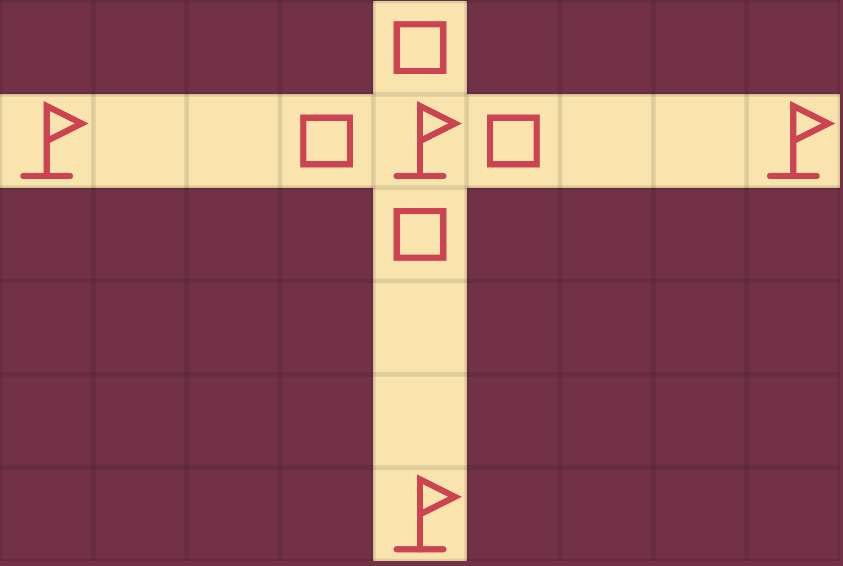
\includegraphics[width=\linewidth]{img/path}
		\caption{Pathological case for ICTS-m}
		\label{fig:path}
	\end{wrapfigure}
	\subsubsection{Pathological case}
	\label{pathology}
	As a consequence of the $\min$ operation in the root definition, a pathological case can be derived. Consider a team of 4 agents $a_1^1$ through $a_4^1$. Let them be arranged in a configuration as depicted in Figure \ref{fig:path}. All four agents match the colour of the centre goal and hence for each $i$, $c^*_i = 1$, so that the root is $(1,1,1,1)$ with SIC $4$. The optimal solution however is, numbering the agents clockwise, $(1,3,3,3)$ with SIC $10$, meaning that $\Delta = 6$. It can be seen that instances of this form with arbitrarily large $\Delta$ can be constructed. As ICTS-m being a generalization of ICTS is $\mathcal{O}(k^\Delta)$, even just extending the 'limbs' of the instance to yield an ICT root of $(1,9,9,9)$ with $\Delta = 24$ will result in an unfathomably large number of nodes being evaluated assuming no pruning or other modifications to the base algorithm.
	%\subsubsection{Inverted MDD search}
	%The uniqueness of goals guarantees the existence of a goal node without vertex conflicts in searching MDDs in MAPF. In MAPFM, this is not the case and causes joint MDDs to be searched fully without finding a result. In addition, even if there exists a goal node, many of the paths represented by the joint MDD lead to conflicting maximal-depth nodes.
	
	%To avoid this, the MDD search could be changed to start at the maximal depth and search for a way towards the start node, which by start uniqueness remains without vertex conflicts.
	%Two strategies could be used to avoid this: firstly, the MDD search could be changed to start at the maximal depth and search for a way towards the start (which by start uniqueness is always non-conflicting); secondly, a bipartite matching algorithm could be employed to see if any matching exists between agents and goals they can reach. An advantage of the former strategy is that it will, in particular with larger team sizes, reduce the number of maximal depth nodes drastically, so that the subsequent search is from few nodes to one goal. By only running a matching algorithm to skip regular MDD search, there is no such reduction so from one starting position paths will be searched to potentially an exponential number of goal nodes, of which many will end up being illegal. 
	%[TODO: just focus on explaining why inverted MDD search was/could be used to solve this? Or just toss this out for lack of time/space. Why didn't I come up with this idea earlier...]
	\subsection{Optimizations}
	To improve both types of algorithms, some optimizations were found that can be used to speed up the search. These are here motivated. 
	\subsubsection{Bounds in ID}
	The information gained about solution costs of independent groups can be used to establish a lower bound on solution SIC as per Property \ref{property:id-lower}. In bounded search, the upper bound can be further constrained by Property \ref{property:id-upper}.
	\begin{property}[Lower bound]
		When merging groups $g_i,g_j$ with solution costs $C_i,C_j$ to yield group $g_k$, for any solution for this group with cost $C_k$
		\[C_k\geq C_i + C_j\]
		\label{property:id-lower}
	\end{property}
	\begin{proof}
		Assume there would be a solution with $C_k < C_i + C_j$. Taking $C_k^i$ to denote the SIC of agents that used to make up $g_i$ in the solution to $g_k$, without loss of generality $C_k^i < C_i$, which contradicts the optimality of the solution with cost $C_i$ for $g_i$ independent of $g_j$.
	\end{proof}
	\begin{property}[Reduced upper bound]
		In bounded exhaustive search, the sum of costs of groups not being merged can be subtracted from bound $B$ without losing optimality.
		\label{property:id-upper}
	\end{property}
	\subsubsection{Child pruning}
	In the original ICTS formulation all $k$-children are generated in every case because pruning only controls skipping the low-level search, assumed to be the most expensive operation. However, in simple pruning in any case, when there is a conflict between two or more agents at a given ICT node $(c_1,\ldots,c_k)$, in any solution, one or more of the path costs corresponding to these conflicting agents will have to be incremented. This can be exploited by pruning the node's children that do not correspond to the conflicting agents, of which there are often just 2 or 3, drastically improving the (average) branching factor as $k$ increases. By Property \ref{property:ec-incompat}, child pruning is not compatible with enhanced pruning.
	\begin{property}[Incompatibility with enhanced pruning]
		Enhanced pruning combined with child pruning is suboptimal due to the \textit{cascading effect} described in \cite{sharon2011}.
		\label{property:ec-incompat}
	\end{property}
	
	\begin{figure}[H]
		\centering
		\begin{subfigure}{0.40\textwidth}
			\centering
			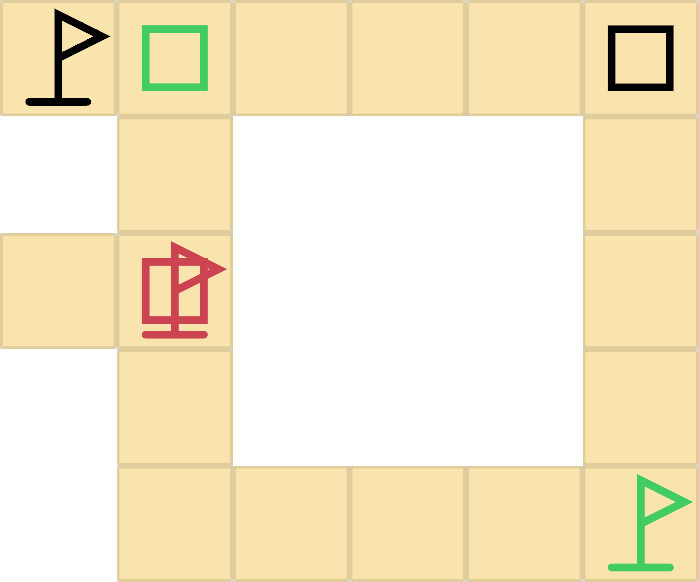
\includegraphics[width=\linewidth]{img/counter-example-ep-2}
			\caption{Instance}
			\label{fig:counter-example:a}
		\end{subfigure}
		\begin{subfigure}{0.49\textwidth}
			\centering
			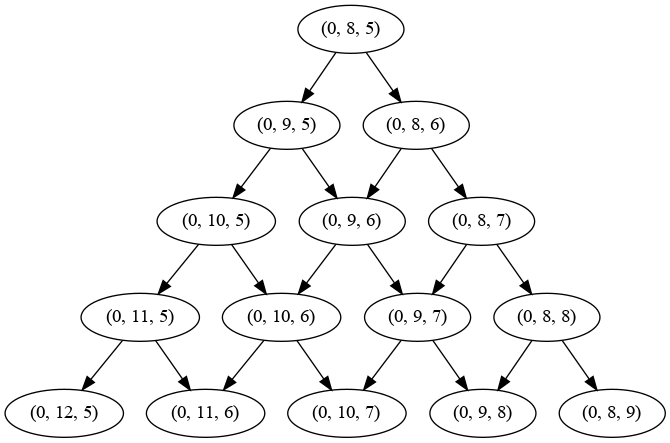
\includegraphics[width=\linewidth]{img/counter-example-tree}
			\caption{Pruned ICT that is traversed}
			\label{fig:counter-example:b}
		\end{subfigure}
		\caption{Counter-example for enhanced pruning combined with child pruning}
		\label{fig:counter-example}
	\end{figure}
	\begin{proof}
		Consider Figure \ref{fig:counter-example:a} with a red agent $r$, green agent $g$ and black agent $b$. It can be seen that $(3,8,5)$ with SIC $16$ is an optimal solution for this instance, which corresponds to $r$ moving aside, allowing $g$ to pass.  Say enhanced pruning with pairs is applied to these three agents at $(c^*_r,c^*_g,c^*_b) = (0,8,5)$. Let the enhanced pruning order be $(r,g)$, $(r,b)$, $(g,b)$ without loss of generality. $(r,g)$ is solvable but will leave for $g$ out of the two paths of length $8$ only the clock-wise path. $(r,b)$ will not change either MDD in this node. When $(g,b)$ is evaluated, it is found that the remaining clockwise path for $g$ and $b$'s path are incompatible (edge conflict) so $(0,9,5)$ and $(0,8,6)$ are generated. By repeating this order of enhanced pruning with child pruning, the ICT shown in \ref{fig:counter-example:b} is traversed. Notice that none of the nodes with SIC 16 in this ICT are a solution, meaning that enhanced pruning combined with child pruning will return a suboptimal solution to the instance in \ref{fig:counter-example:a}, making this pruning strategy suboptimal.
	\end{proof}
	
	\section{Experimental Results}
	\label{experiments}
	To compare the algorithms and variants described above with each other and with alternative MAPFM algorithms, two types of experiments were performed. In the first, ICTS-based algorithms discussed in this work are compared; in the second, the approximate ordered enumeration variant is compared to other algorithms for MAPFM developed within the peer group. This comparison data originates in \cite{donszelmann2021}. The values compared are the fraction of instances solved, and the average runtime per instance. It should be noticed that in the latter, the recorded runtimes converge to the 120s timeout used as fewer instances are solved; therefore, while the times are included for completeness at the end of this work (Figure \ref{fig:i-times} and \ref{fig:r-times} for experiments 1 and 2), the fraction of instances solved is guiding in the analysis of results.
	\newgeometry{left=1cm,right=1cm,top=0.1cm,bottom=0.1cm}
	\begin{figure*}[t]
		\centering
		\begin{subfigure}{0.44\textwidth}
			\centering
			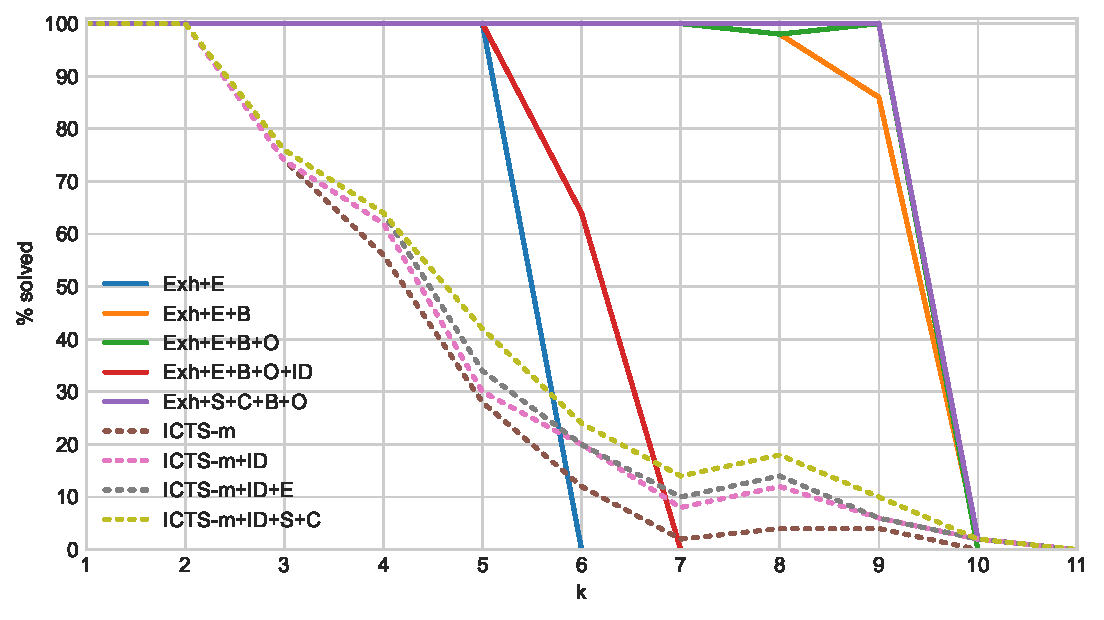
\includegraphics[width=\linewidth]{img/results/icts-comparison/25-1-p}
			\caption{25\% wall, 1 team}
			\label{fig:i-25-1-p}
		\end{subfigure}
		\begin{subfigure}{0.44\textwidth}
			\centering
			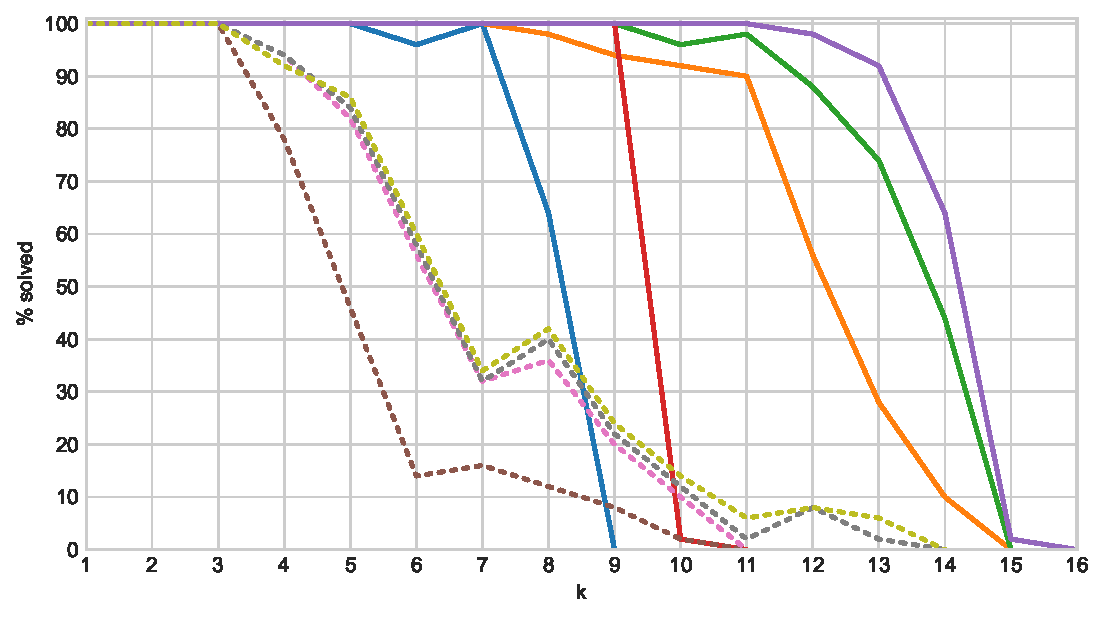
\includegraphics[width=\linewidth]{img/results/icts-comparison/25-3-p}
			\caption{25\% wall, 3 teams}
			\label{fig:i-25-3-p}
		\end{subfigure}
		\begin{subfigure}{0.44\textwidth}
			\centering
			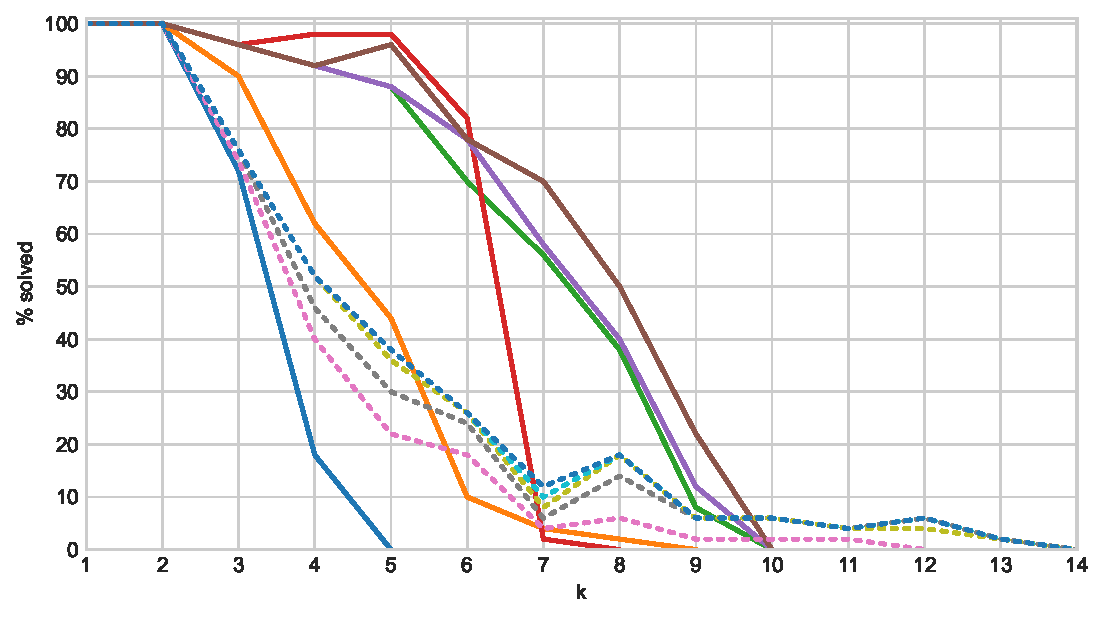
\includegraphics[width=\linewidth]{img/results/icts-comparison/75-1-p}
			\caption{75\% wall, 1 team}
			\label{fig:i-75-1-p}
		\end{subfigure}
		\begin{subfigure}{0.44\textwidth}
			\centering
			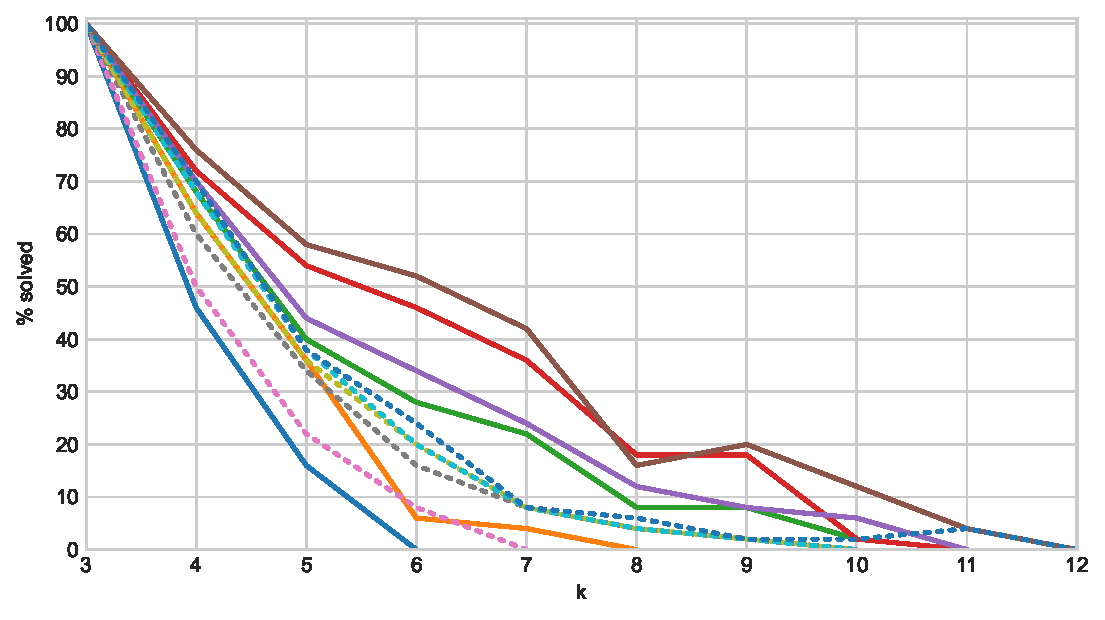
\includegraphics[width=\linewidth]{img/results/icts-comparison/75-3-p}
			\caption{75\% wall, 3 teams}
			\label{fig:i-75-3-p}
		\end{subfigure}
		\caption{Fraction solved out of 50 maps by different ICTS-based algorithms}
		\label{fig:i-probs}
	\end{figure*}
	\begin{figure*}[b]
		\centering
		\begin{subfigure}{0.44\textwidth}
			\centering
			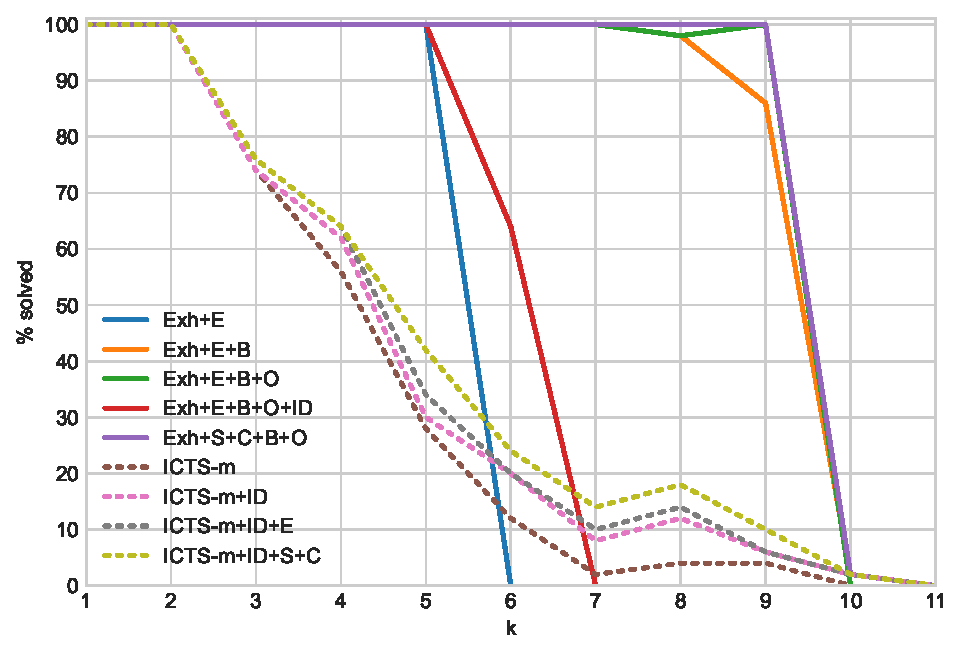
\includegraphics[width=\linewidth]{img/results/relative-comparison/25-1-p}
			\caption{25\% wall, 1 team}
			\label{fig:r-25-1-p}
		\end{subfigure}
		\begin{subfigure}{0.44\textwidth}
			\centering
			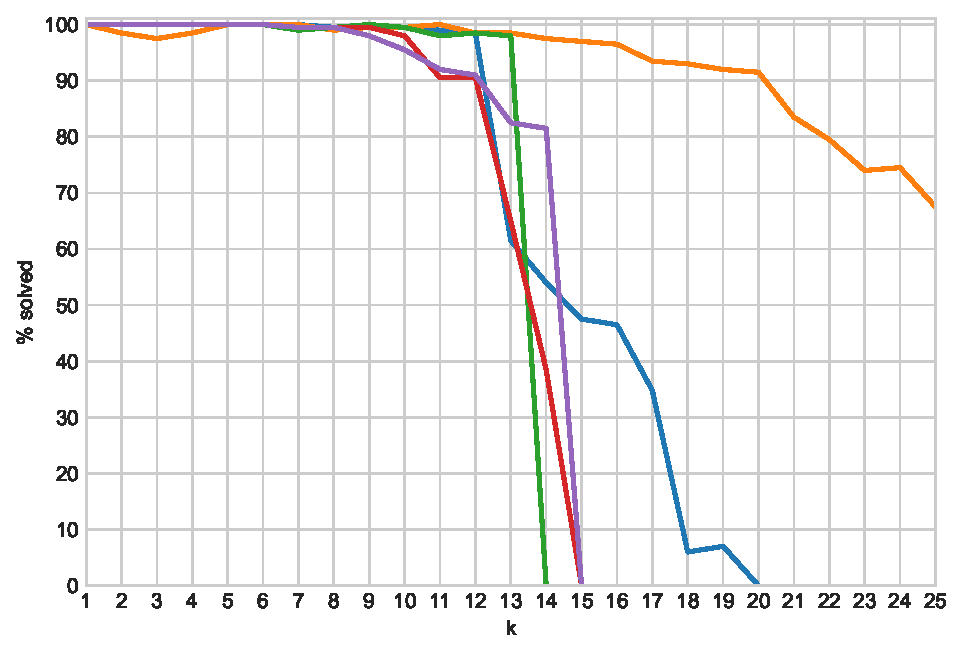
\includegraphics[width=\linewidth]{img/results/relative-comparison/25-3-p}
			\caption{25\% wall, 3 teams}
			\label{fig:r-25-3-p}
		\end{subfigure}
		\begin{subfigure}{0.44\textwidth}
			\centering
			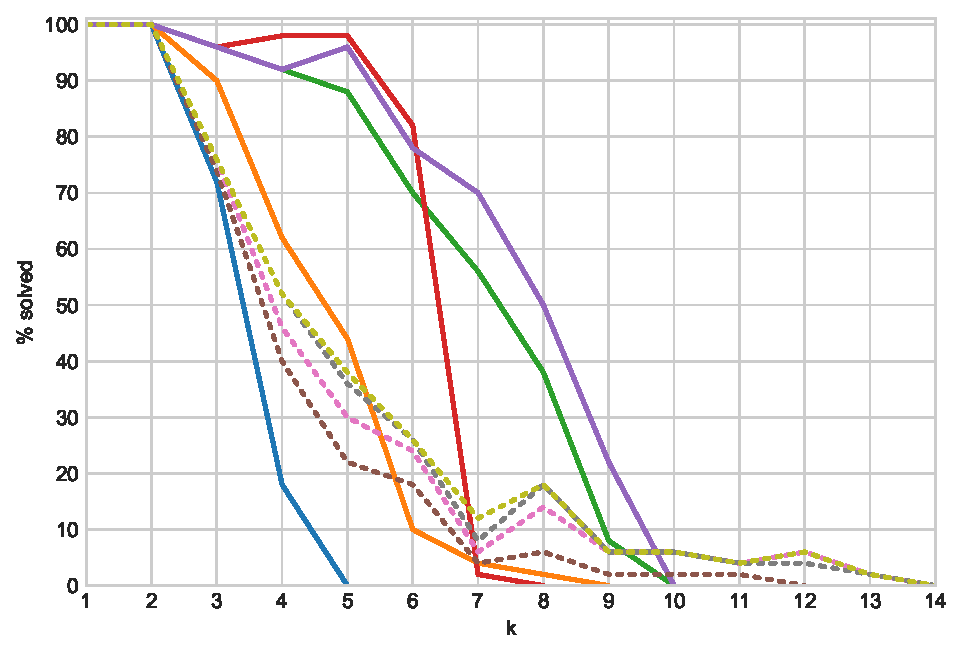
\includegraphics[width=\linewidth]{img/results/relative-comparison/75-1-p}
			\caption{75\% wall, 1 team}
			\label{fig:r-75-1-p}
		\end{subfigure}
		\begin{subfigure}{0.44\textwidth}
			\centering
			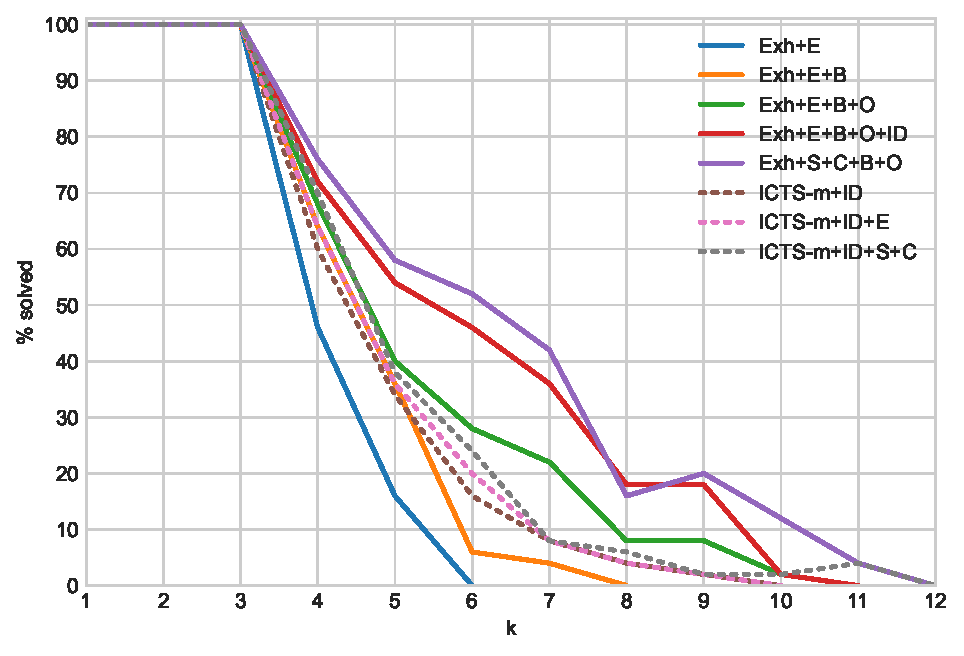
\includegraphics[width=\linewidth]{img/results/relative-comparison/75-3-p}
			\caption{75\% wall, 3 teams}
			\label{fig:r-75-3-p}
		\end{subfigure}
		\caption{Fraction solved out of 200 maps by MAPFM algorithms}
		\label{fig:r-probs}
	\end{figure*}
	
	\restoregeometry
	\subsection{Experimental setup}
	Because MAPFM lies on the fringe of pathfinding research, no standard benchmark exists. For MAPF, the Moving AI benchmarks \cite{sturtevant2012} are often used and potentially a new MAPFM standard benchmark could be defined by generating suitable team-partitions of agents for these MAPF instances; however, it was noticed that optimally solving even small MAPFM instances with comparatively few agents and short distances to goals was already a challenge computationally. This observation informed the creation of a map generator by the author of \cite{jong2021} with various parameters. Using this map generator, two types of 20x20 grids were generated:
	\begin{enumerate}
		\item 25\% wall: a grid with 25\% of tiles being obstacles.
		\item 75\% wall: a grid with 75\% of tiles being obstacles. 
	\end{enumerate}
	For each of these types, maps were generated with between $1$ and $25$ agents either all in the same team or partitioned into $3$ teams as fairly as possible. When solving the instances, for each combination of map-type and number of teams, the number of agents was increased until 0\% of instances could be solved within a timeout of 120s, at which point no more data was recorded for greater numbers of agents.
	
	The first experiments were performed on an Intel i7-8750H hexacore operating at 2.2GHz with 16GiB of memory. For each setting, a fixed subset of 50 out of 200 maps were used. Hyperthreading was used in experiments, but because agent-settings were solved in sequence as batches, it is expected that this has affected experimental outcomes equally.
	
	The second experiments comparing the different MAPFM algorithms within the peer group were run on a server with a virtualized Intel Xeon E5-2683 dodecacore operating at 2.0Ghz with 8GiB of RAM. All 200 maps were used for each setting.
	
	All algorithms are implemented in Python 3.9 to avoid performance differences as often seen between interpreted versus compiled languages; however, CBM\cite{baauw2021} in experiment 2 does use an SSP solver implemented in C++ as a subroutine. Nonetheless, the comparison in this experiment is more coarse-grained as performance differences are sometimes subtle and could potentially be explained by slight implementation optimizations rather than algorithmic properties.
	
	\subsection{Experiment 1: ICTS-based MAPFM algorithms}
	To investigate the relative performance of various algorithms discussed in Section \ref{section:icts-matching}, a selection of both exhaustive and ICTS-m variants was made. Their performance in terms of fraction of problems solved within a timeout of 120s is shown in Figure \ref{fig:i-probs}. The meaning of the abbreviations used in the legend are as follows:
	\begin{itemize}
		\begin{minipage}{0.45\linewidth}
			\item S: Simple pruning
			\item E: Enhanced pruning
			\item C: Child pruning
		\end{minipage}
		\begin{minipage}{0.45\linewidth}
			\item ID: Independence detection
			\item B: Bounded search
			\item O: Approximate ordered enumeration
		\end{minipage}
	\end{itemize}
	Across scenarios, it is seen that typically exhaustive methods outperform ICTS-m algorithms (\ref{fig:i-probs}), with performance being more similar in the maps with 75\% wall. In particular on 75\% wall maps with 3 teams (\ref{fig:i-75-3-p}), the performance of ICTS-m+ID (and optional pruning) is seen to outperform bounded exhaustive search as $k$ increases, and some of these also manage to solve a small fraction of 75\% maps with 1 team that exhaustive methods cannot within the time-out (\ref{fig:i-75-1-p}).
	
	Between exhaustive variants, with exception of the ID variant, a type of hierarchy can be distinguished, best illustrated by \ref{fig:i-25-3-p}; almost without exception, Exh+S+C+B+O outperforms Exh+E+B+O which outperforms Exh+E+B which in turn outperforms Exh+E. Bounded search outperforms unbounded search as expected, given that the former does at most as much work as the latter and often less. Approximate ordering outperforming unordered enumeration is not quite as obvious from a theoretical standpoint, as discussed in \ref{ordered-enum}, and simply indicates that sorting works well in practice. Simple pruning with child pruning outperforming exhaustive pruning shows the potential of this pruning method. In particular, as $k$ grows larger and in scenarios with more obstacles (\ref{fig:i-75-1-p},\ref{fig:i-75-3-p}), it appears that having to search a smaller ICT is more important in terms of performance than being able to skip the $k$-agent low-level search more often. As discussed in Section \ref{future}, more work is needed to determine if such an improvement is to be expected more generally.
	
	The benefit of using ID together with ordered enumeration is less clear. Ordered enumeration with ID performs much better in \ref{fig:i-75-3-p}, a setting with more obstacles and more teams, but ordered enumeration without ID on the other hand is superior in an open setting with a single team (\ref{fig:i-25-1-p}). The overhead associated with the various planning and merging steps (see Algorithm \ref{id-algo}) could be the cause the slowdown observed once $M$ grows large (\ref{fig:i-25-1-p},\ref{fig:i-75-1-p}); once the upper bound is tightened, ICTs only have to be searched shallowly so there is no point in going through the steps of ID. This explains why no speedup is seen, as ICTS-m between and ICTS-m+ID. Another factor is that if all agents belong to the same team, it is somewhat unlikely that there will a significant benefit to using ID, as agents from the same team planned independently often route to the same goal.
	
	\subsection{Experiment 2: Algorithms for MAPFM}
	From the variants discussed and compared above, the Exh+E+B+O variant was selected for comparison with various other algorithms for MAPFM. This results in the following set of algorithms whose performance is shown in Figure \ref{fig:r-probs}.
	\begin{itemize}
		\begin{minipage}{0.45\linewidth}
			\item ICTS with approximate sorted exhaustive matching (Exh+E+B+O)
			\item A*+ID+OD with matching ID and sorted exhaustive matching\cite{bruin2021}
			\item EPEA* with matching ID and sorted exhaustive matching\cite{jong2021}
		\end{minipage}
		\hspace{1cm}
		\begin{minipage}{0.40\linewidth}
			\item M* with sorted exhaustive matching\cite{donszelmann2021}
			\item CBM adapted to use SIC, using the successive shortest path algorithm (SSP) \cite{goldberg1987} as subroutine for solving teams\cite{baauw2021}.
		\end{minipage}
	\end{itemize}
	With exception of CBM, all methods described use a variant of sorted exhaustive matching. This is because from each family of algorithms one of the best performing algorithms was chosen, which always was such an exhaustive method as opposed to a generalization of the base algorithm to MAPFM (ICTS-m in this work). A*+ID+OD and EPEA * also make use of matching ID, which is ID applied to the MAPFM instance using the respective exhaustive algorithm as MAPFM solver. Hypothetically, this could explain why both outperform the methods using just sorted exhaustive matching in maps with 75\% wall and 3 teams (\ref{fig:r-75-3-p}); this difference is not quite as clear in the remaining scenarios shown in Figure \ref{fig:r-probs} however. 
	
	CBM solving all problems with one team (Figure \ref{fig:r-25-1-p} and \ref{fig:r-75-1-p}), problems equivalent to anonymous MAPF instances, is at first surprising but follows directly from the definition of the CBM method. CBM solves single teams as anonymous MAPF instances in polynomial time, meaning that solving a single team reduces to a polynomial-time procedure, namely SSP. Following the results reported in \cite{ma2016}, it is expected that as the number of teams approaches $k$, CBM performance will deteriorate and thus become more similar to the results for exhaustive methods here reported. As CBM is based on CBS, scenarios such as mazes with even more obstacles and potentially conflicts would also be interesting to consider in comparison of CBM to the exhaustive methods.
	%	Still, some implementations might be more optimized than others so this might be a factor in performance characteristics and in particular in relative performance differences.
	\section{Conclusions and Future work}
	\label{conclusions}
	\label{future}
	The goal of this research was to seek alternative approaches to solving MAPFM based on ICTS. In this, the research has succeeded, but the scalability of the algorithms leaves something to be desired. Exhaustive methods, like those discussed in detail in \ref{exhaustive}, cannot be expected to scale well as teams grow larger due to their complexity, no matter what optimizations are put in place. Nonetheless, as was shown in Section \ref{experiments}, the more advanced exhaustive ICTS algorithms consistently outperform the ICTS-m based algorithms. Compared to the SIC-adaptation of the CBM method \cite{baauw2021}, it was seen that exhaustive methods generally perform quite poorly if there are fewer teams and fewer obstacles, while being competitive once teams grow smaller and maps become more constrained. Delineating under which conditions exhaustive methods outperform CBM and vice versa is something for further research.
	
	Future research could also look into improving the ICTS-m method described using for instance more extensive pruning or properties of the problem such as lower-bounds on per-team solution SIC that can be computed using the Hungarian Algorithm. Another approach to explore would be hybridized approaches that enumerate partially constrained MAPFM instances which can be solved using any MAPFM solver. In this way, the benefit of the successive bounding of the search could be exploited and by carefully picking which agents to constrain, these constrained MAPFM instances could potentially be made relatively easy.
	
	Lastly, more experimentation is needed to reach definite conclusions about how simple child pruning compares to existing pruning techniques for ICTS, which could be done by reproducing the ICTS pruning technique experiments reported in \cite{sharon2011} extended with simple child pruning variants. %Given that simple pruning is somewhat cheap computationally, it might also be possible to prune the child generation using simple child pruning but still use enhanced pruning to decide whether to execute $k$-agent low-level search, combining the benefits of searching a smaller ICT and performing fewer $k$-agent searches.
	
	\section{Responsible Research}
	The implementation of the ICTS-based algorithms described in this work is publicly available online in the form of a Github repository\footnote{\url{https://github.com/tbvanderwoude/icts-m}}. Included is also code for benchmarking different configurations of the ICTS solver and the maps that were used in the benchmarks reported above. The benchmarks and maps used in the relative comparison of MAPFM algorithms are also available in the code and data repository of \cite{donszelmann2021}\footnote{\url{https://github.com/jonay2000/research-project}}.
	
	\printbibliography
	\newgeometry{left=1cm,right=1cm,top=0.1cm,bottom=0.1cm}
	\begin{figure*}[t]
		\centering
		\begin{subfigure}{0.44\textwidth}
			\centering
			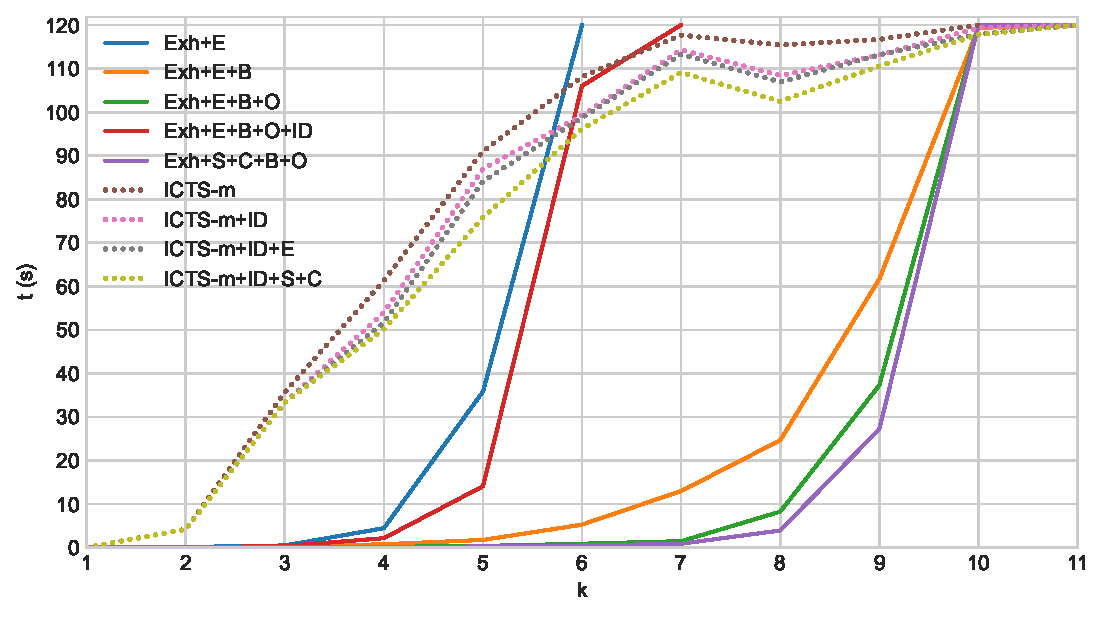
\includegraphics[width=\linewidth]{img/results/icts-comparison/25-1}
			\caption{25\% wall, 1 team}
			\label{fig:i-25-1}
		\end{subfigure}
		\begin{subfigure}{0.44\textwidth}
			\centering
			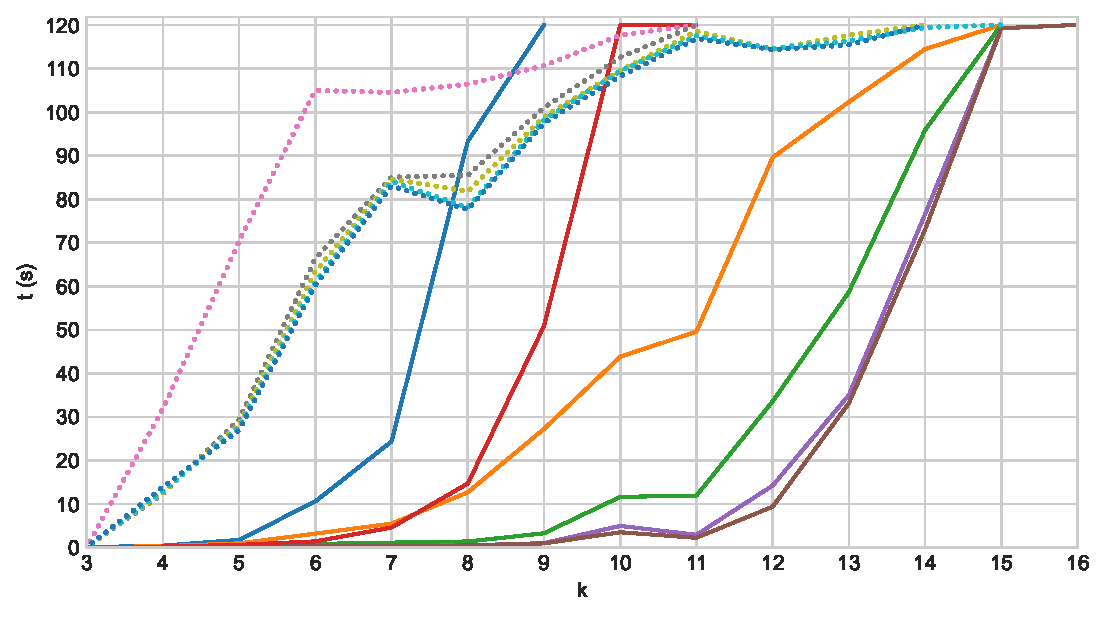
\includegraphics[width=\linewidth]{img/results/icts-comparison/25-3}
			\caption{25\% wall, 3 teams}
			\label{fig:i-25-3}
		\end{subfigure}
		\begin{subfigure}{0.44\textwidth}
			\centering
			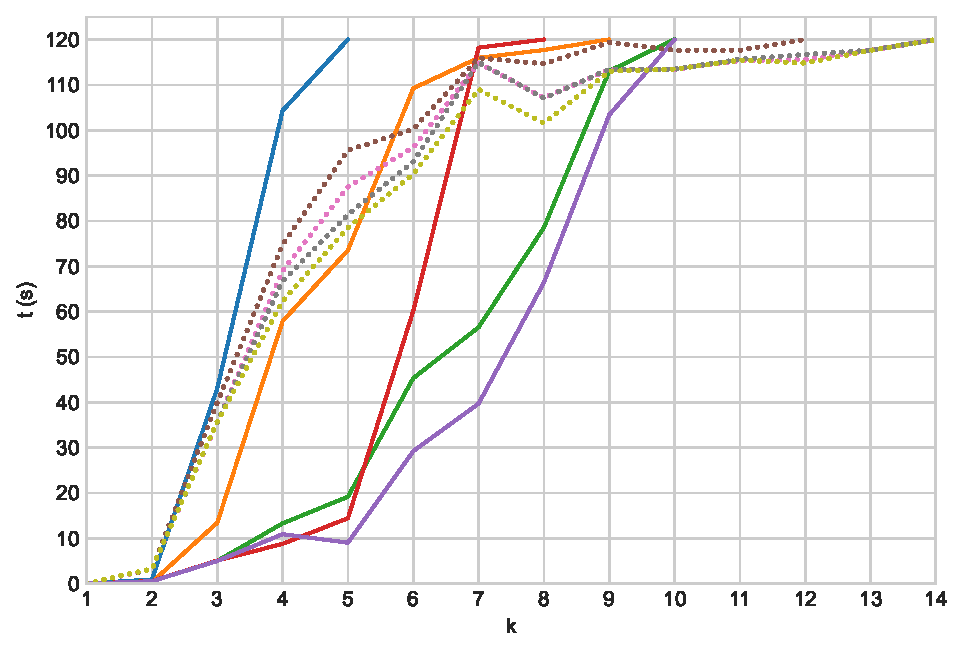
\includegraphics[width=\linewidth]{img/results/icts-comparison/75-1}
			\caption{75\% wall, 1 team}
			\label{fig:i-75-1}
		\end{subfigure}
		\begin{subfigure}{0.44\textwidth}
			\centering
			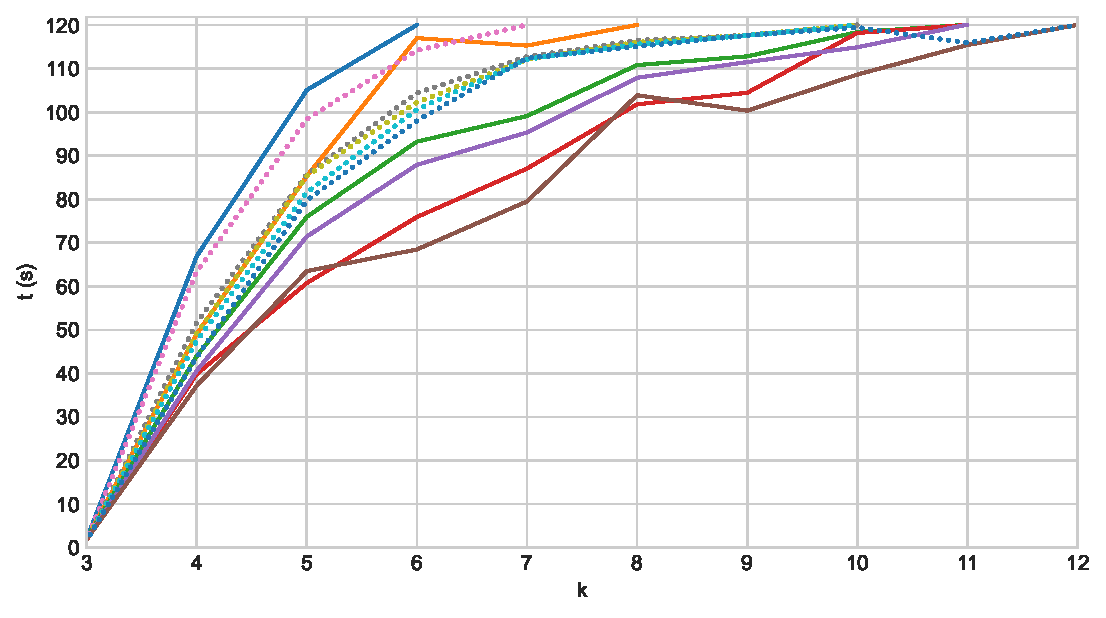
\includegraphics[width=\linewidth]{img/results/icts-comparison/75-3}
			\caption{75\% wall, 3 teams}
			\label{fig:i-75-3}
		\end{subfigure}
		\caption{Average solving time of different ICTS-based algorithms with a timeout of 120s}
		\label{fig:i-times}
	\end{figure*}
	\begin{figure*}[b]
		\centering
		\begin{subfigure}{0.44\textwidth}
			\centering
			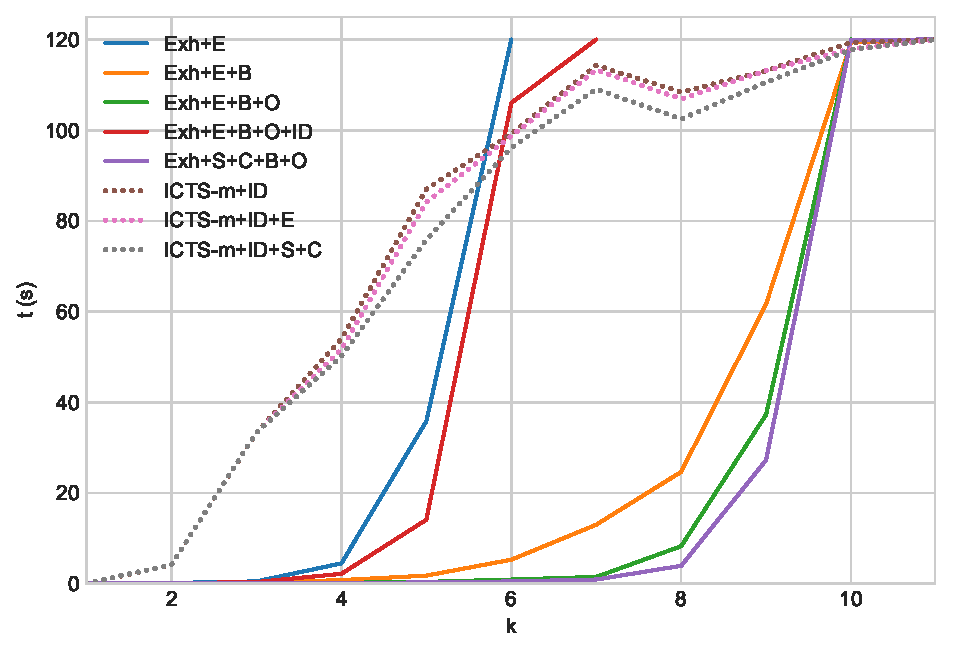
\includegraphics[width=\linewidth]{img/results/relative-comparison/25-1}
			\caption{25\% wall, 1 team}
			\label{fig:r-25-1}
		\end{subfigure}
		\begin{subfigure}{0.44\textwidth}
			\centering
			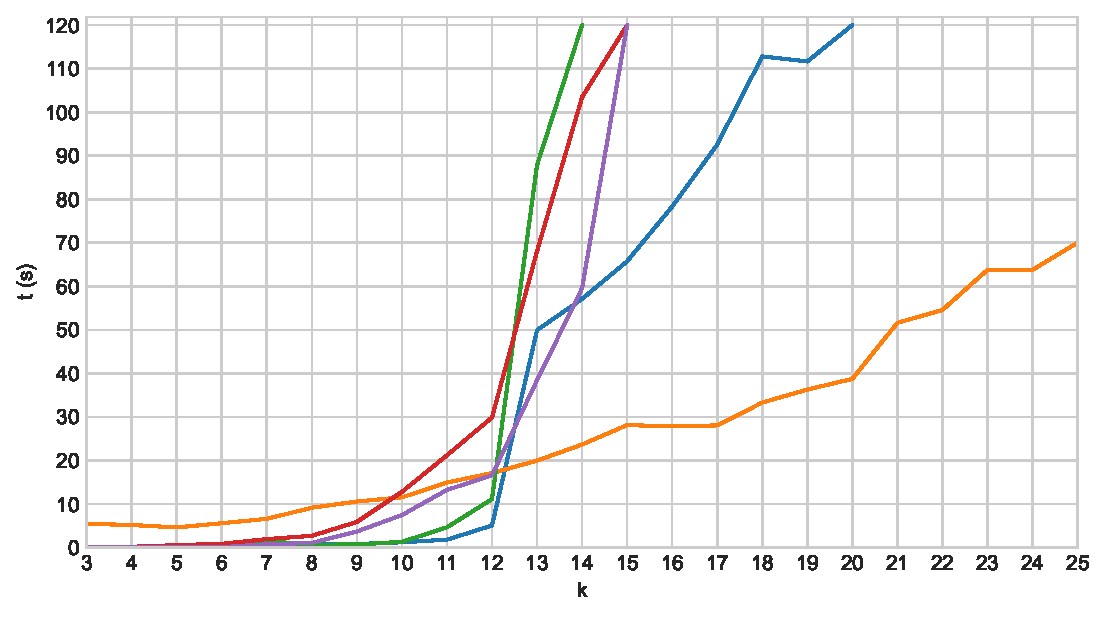
\includegraphics[width=\linewidth]{img/results/relative-comparison/25-3}
			\caption{25\% wall, 3 teams}
			\label{fig:r-25-3}
		\end{subfigure}
		\begin{subfigure}{0.44\textwidth}
			\centering
			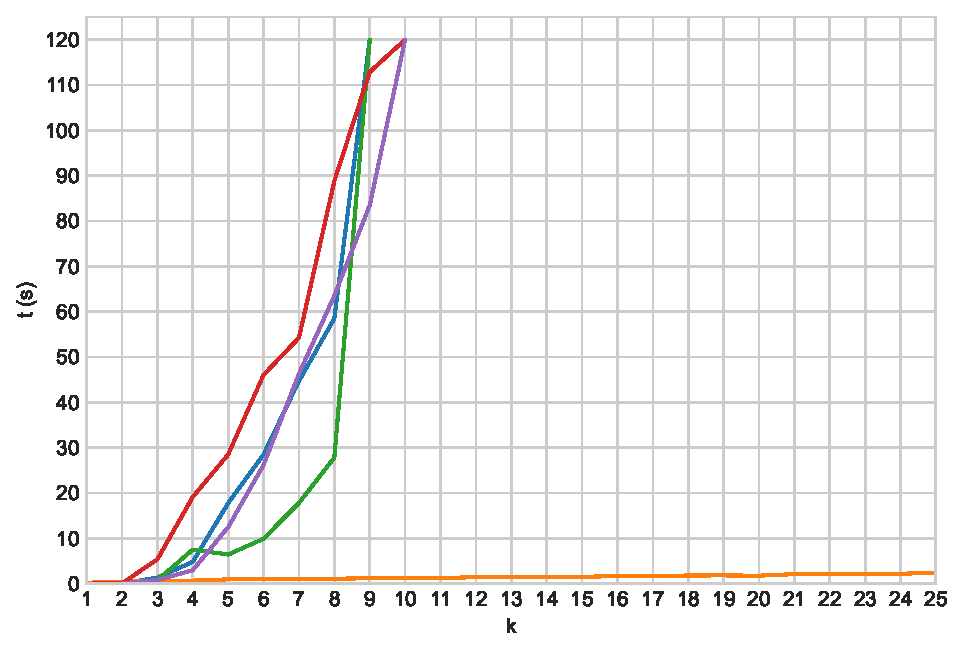
\includegraphics[width=\linewidth]{img/results/relative-comparison/75-1}
			\caption{75\% wall, 1 team}
			\label{fig:r-75-1}
		\end{subfigure}
		\begin{subfigure}{0.44\textwidth}
			\centering
			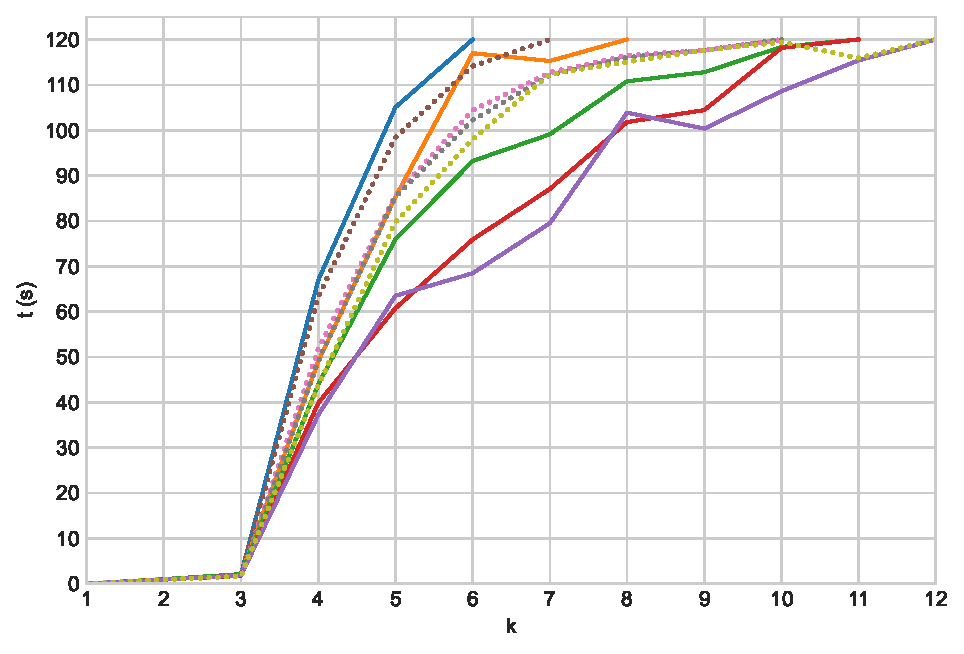
\includegraphics[width=\linewidth]{img/results/relative-comparison/75-3}
			\caption{75\% wall, 3 teams}
			\label{fig:r-75-3}
		\end{subfigure}
		\caption{Average solving time of MAPFM algorithms with a timeout of 120s}
		\label{fig:r-times}
	\end{figure*}
	
	\restoregeometry
\end{document}
